% -*- coding: utf-8; mode: latex; -*-

%
% NTT Tech Conference 2025
% Showcase/Lightning Talks
% 「演奏間違いを検出して楽譜上に指摘の表示をしてみる」
% https://github.com/trueroad/tr-NTTtech2025
%
% 発表資料のソース(配布版)
%
% Copyright (C) 2025 Masamichi Hosoda.
% This file is licensed under a Creative Commons Attribution-ShareAlike 4.0
% International License.
%

% +++
% latex = "lualatex"
% extra_clean_files = ["%B.xmpdata", "pdfa.xmpi", "%B.ltjruby"]
% +++

% PDF/A のメタデータ(pdfx.sty が読み込む)
\begin{filecontents*}{\jobname.xmpdata}
  \Language{ja-JP}
  \Title{演奏間違いを検出して楽譜上に指摘の表示をしてみる}
  \Author{細田 真道}
  \Subject{NTT Tech Conference 2025}
  \Copyright{%
    Copyright (C) 2024 Masamichi Hosoda.
    This paper is licensed under a Creative Commons Attribution-ShareAlike 4.0
    International License.}
  \Creator{% ここで設定してやらないと(自動設定や \hypersetup だと)化ける
    LaTeX with Beamer class}
\end{filecontents*}

% LuaTeX マニュアルより、出力しないものを指定
% ただし ID を出力しないと PDF/A-2 Rule 6.1.3-1 違反になる
% Creator, CreationDate, ModDate, Producer, Trappedは
% ナゼか出力抑制できない模様なのでそのまにする
\pdfvariable suppressoptionalinfo \numexpr
        0
%    +   1   % PTEX.FullBanner
    +   2   % PTEX.FileName
    +   4   % PTEX.PageNumber
    +   8   % PTEX.InfoDict
%    +  16   % Creator
%    +  32   % CreationDate
%    +  64   % ModDate
%    + 128   % Producer
%    + 256   % Trapped
%    + 512   % ID
\relax

%
% クラスファイル読み込み
%

% beamer を使う
\documentclass[%
  aspectratio=169,% 縦横比16:9
  unicode,%
  17pt,%
  hyperref={pdfa},% beamer は hyperref を読み込むので PDF/A のために必要
]{beamer}

%
% フォントなどの指定(LuaLaTeX 向け)
%

% LuaTeX-ja を使う
\usepackage{luatexja}

%
% フォントなどの指定(LuaLaTeX 向け)
%

% ルビ用
\usepackage{luatexja-ruby}

% 欧文・数式フォント設定の事前準備
\usepackage[no-math]{fontspec}

% 和文フォント設定
\usepackage[%
  deluxe,%         複数のウェイトを使う
  match,%          欧文フォントのファミリ指定と連動させる
  nfssonly,%       luatexja-fontspec を使わない(メモリ・時間節約)
  haranoaji%       原ノ味フォントを指定
]{luatexja-preset}

% 和文フォントの既定をゴシックに
\renewcommand{\kanjifamilydefault}{\gtdefault}

% 欧文フォント設定
\setmainfont{Libertinus Serif}
\setsansfont{Libertinus Sans}
\setmonofont{Source Code Pro}[Scale=MatchLowercase]% 大きく見えるので調整

% LuaTeX-ja 調整
\usepackage{luatexja-adjust}
\ltjenableadjust[%
  lineend=extended,% 行末文字の位置調整    : 行分割の過程で考慮
  priority=true,%    優先順位付きの行長調整: 有効化
  profile=true%      中身まで見た行送り計算: 有効化
]

% pdfx.sty で PDF バージョン指定が効かない対策
\usepackage{luatex85}

%
% 各種パッケージの読み込みと設定
%

\usepackage{tcolorbox}% 枠囲み用
\usepackage{tikz}
\usetikzlibrary{shapes.arrows}% ブロック矢印用
\usepackage[absolute,overlay]{textpos}% 座標指定用
\usepackage{qrcode}% 二次元コード表示用

%
% PDF/A 関連設定
%

% pdfx.sty で PDF/A-2u の作成を指定
\usepackage[%
  pdf15,% PDF 1.5 の生成を指定
  a-2u%   PDF/A-2u の生成を指定
]{pdfx}

% pdfx.sty が変更した xcolor の設定を再設定
% gray は gray のままで rgb に変換されないようにする
\selectcolormodel{natural}

% 本文を rgb ではなく gray の黒に設定
% gray でも PDF/A-2 的には OK だし、黒はちゃんと黒にしたい
\color[gray]{0}

%
% beamer の設定
%

% スライドのデザイン
\useinnertheme{rounded}
\useoutertheme{infolines}
\usecolortheme[rgb={0.0,0.5,0.0}]{structure}
\usecolortheme{lily}
\usecolortheme{dolphin}
\setbeamertemplate{navigation symbols}{}

% スライドの背景画像
\usebackgroundtemplate{\includegraphics[height=\paperheight]%
  {none-background.png}}

% フォント関連
\usefonttheme{structurebold} % タイトル部を太字
\setbeamerfont{alerted text}{series=\bfseries} % Alertを太字
\setbeamerfont{section in toc}{series=\mdseries} % 目次は太字にしない
\setbeamerfont{date}{size=\small}  % 日付文字サイズ

% 目次に節番号をつける
\setbeamertemplate{section in toc}[sections numbered]

%
% タイトル
%

\title[演奏間違いを検出し楽譜上に指摘表示]{%
  \Large 演奏間違いを検出して \\ 楽譜上に指摘の表示をしてみる}
\author{細田 真道}
\institute[]{\url{https://www.trueroad.jp}}
\date[2025-03-05]{2025年3月5日}

\begin{document}

\begin{frame}
  \titlepage
  \begin{textblock*}{0.5\linewidth}(240pt,1pt)
    \begin{flushright}
      \tiny
      \href{https://ntt-developers.github.io/ntt-tech-conference/2025/}%
           {NTT Tech Conference 2025} Showcase/Lightning Talks \\
      Copyright (C) 2025 Masamichi Hosoda \\
      \href{https://creativecommons.org/licenses/by-sa/4.0/deed.ja}%
           {\includegraphics[height=2.5ex]{by-sa}}
    \end{flushright}
  \end{textblock*}
\end{frame}

\section*{自己紹介}
\begin{frame}\frametitle{自己紹介:%
    \normalfont\color[gray]{0}\ruby{細田}{ほそだ} \ruby{真道}{まさみち}}
  \small NTT グループのどこかでデータドリブンな仕事をしていますが、\\
  今回は仕事ではなく個人的にやっていることをご紹介します
  \begin{itemize}
    \small
  \item \href{http://lilypond.org/}{楽譜作成プログラムLilyPond}コミッタ
  \item \href{https://www.gnu.org/software/texinfo/}
    {GNU公式文書フォーマットTexinfo}コミッタ
  \item \href{https://github.com/trueroad/HaranoAjiFonts}
    {\ruby{原ノ味}{はらのあじ}フォント}主宰
    \begin{itemize}
      \footnotesize
      \item
        \href{https://texjp.org/}{日本語\TeX}デフォルト和文フォント(2020~)
      \item この資料も\TeX で作成、和文は原ノ味フォント
    \end{itemize}
  \end{itemize}

  \footnotesize
  \url{https://github.com/trueroad} \\
  \url{https://researchmap.jp/trueroad} \\
  \url{https://www.trueroad.jp}

  \begin{textblock*}{0.5\linewidth}(335pt,135pt)
    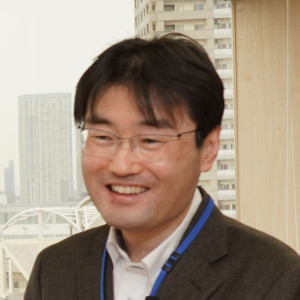
\includegraphics[width=100pt]{20240311_hosoda_face_NTTtech2024.jpg}
  \end{textblock*}
\end{frame}

\section{はじめに}

\begin{frame}\frametitle{はじめに}
  \begin{itemize}
  \item 楽器練習中に自分の演奏が正しいか分からない
    \begin{itemize}
    \item 初心者にはありがち
    \end{itemize}
  \item 自宅練習だと指導者がいない
    \begin{itemize}
    \item 指導者なら指摘できるけど自分ではわからない
    \end{itemize}
  \item 間違った練習を続けて上達の妨げになる

    \vspace{1\zh}
  \item これを解決するツールを作ってみた!
    \begin{itemize}
    \item 演奏間違いを検出
    \item 楽譜上で指摘表示
    \end{itemize}
  \end{itemize}
\end{frame}

\section{しくみ}

\begin{frame}\frametitle{しくみ}
  \begin{itemize}
  \item 演奏情報をMIDIで取得する
    \begin{itemize}
    \item いつ、どの鍵盤を、どんな強さで打鍵したか、離したか \\
      のデータが得られる
    \end{itemize}
  \item 模範演奏データと比較して間違いを検出
  \item 楽譜の上に指摘を重ねて表示
  \end{itemize}
\end{frame}

\section{使い方}

\begin{frame}\frametitle{使い方:%
    \normalfont\color[gray]{0}起動・接続・楽譜選択}
  \centering
  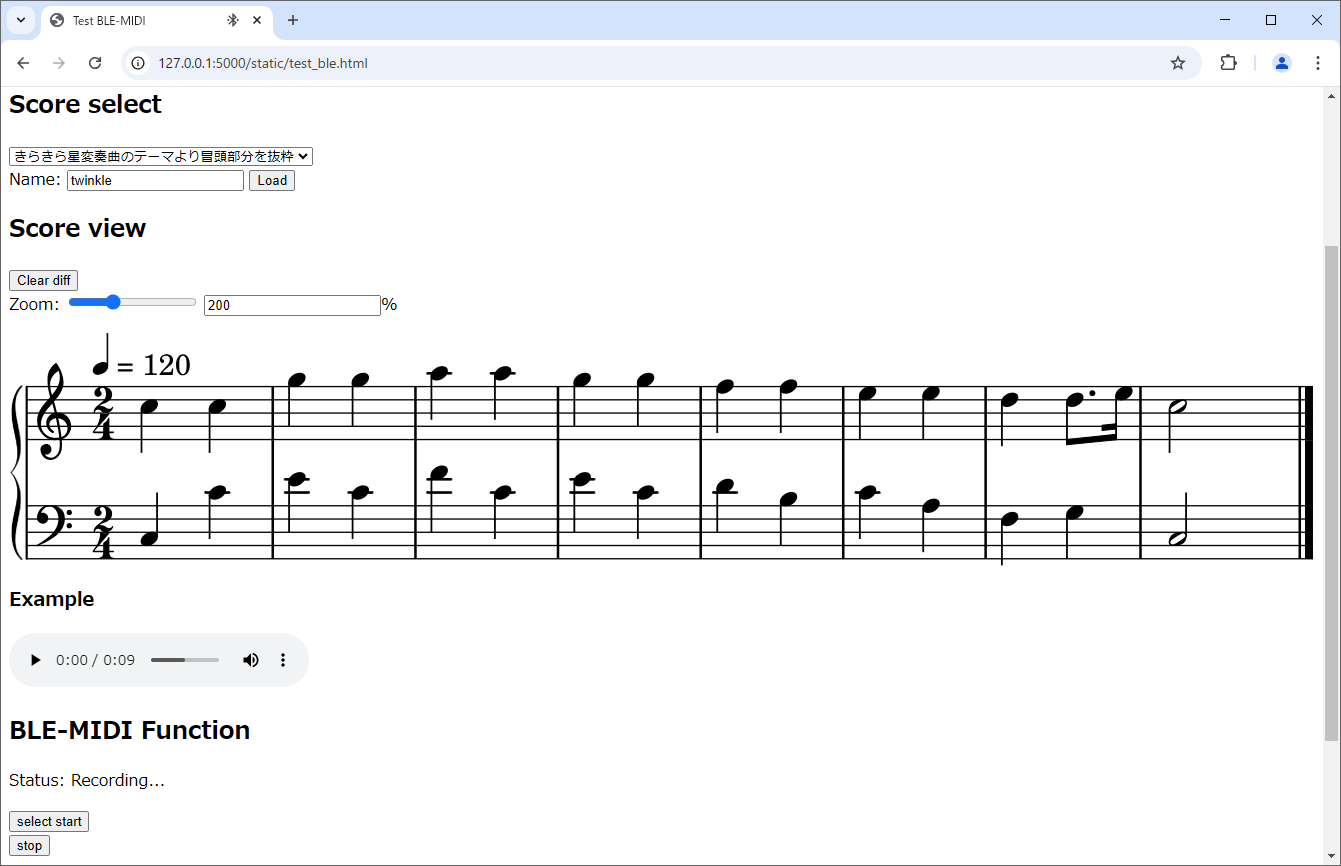
\includegraphics[width=0.7\linewidth]{twinkle-selected.png}

  \begin{textblock*}{0.5\linewidth}(200pt,180pt)
    \onslide<2>{
      \begin{tcolorbox}[width=\linewidth,%
          left=0mm,right=0mm,top=0mm,bottom=0mm,%
          colframe=structure.fg,colbacktitle=structure.fg,%
          colback=structure.bg]
        \centering
        楽譜が表示される
      \end{tcolorbox}
    }
  \end{textblock*}
\end{frame}

\begin{frame}\frametitle{使い方:%
    \normalfont\color[gray]{0}そのまま演奏すると}
  \centering
  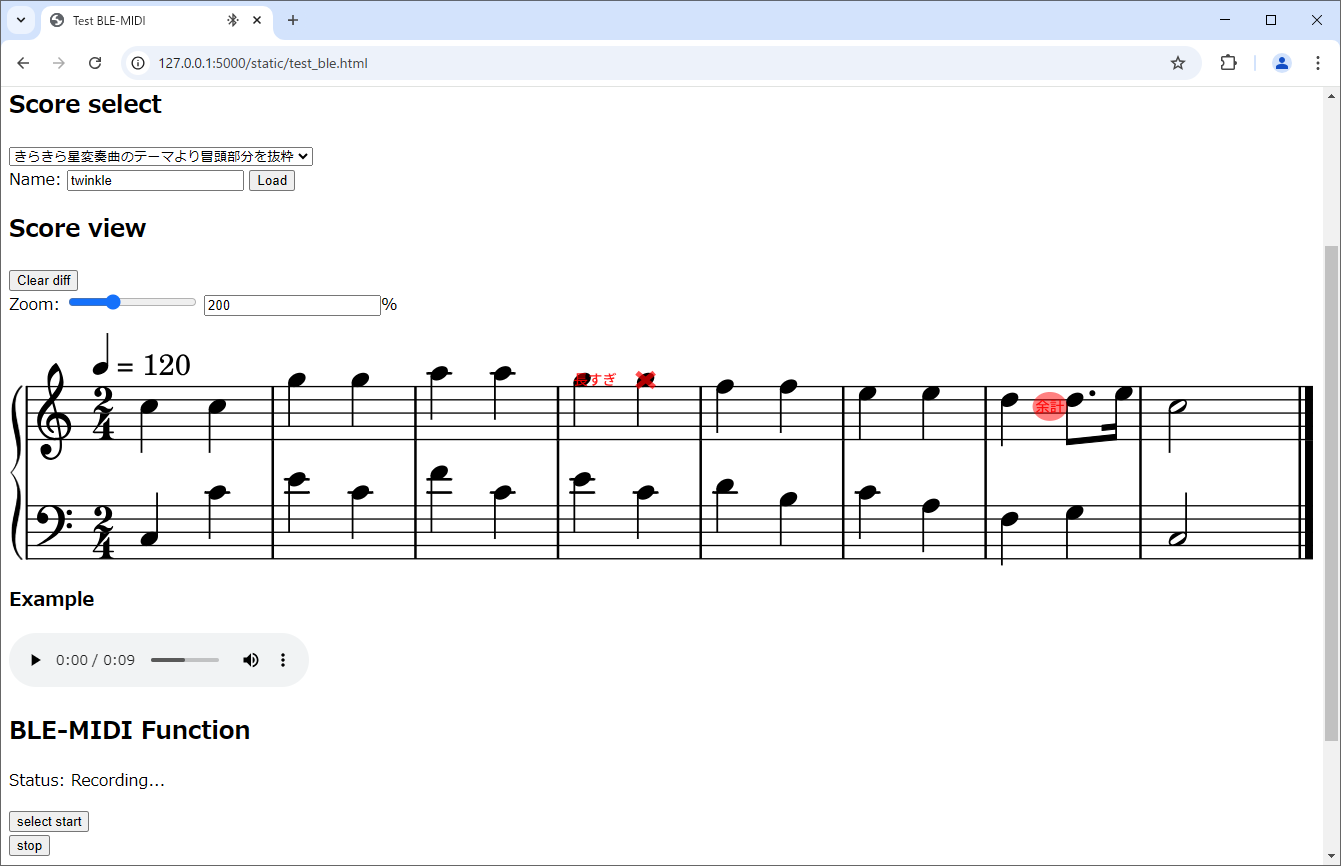
\includegraphics[width=0.7\linewidth]{twinkle-altered-played.png}

  \begin{textblock*}{0.5\linewidth}(200pt,170pt)
    \onslide<2->{
      \begin{tcolorbox}[width=\linewidth,%
          left=0mm,right=0mm,top=0mm,bottom=0mm,%
          colframe=structure.fg,colbacktitle=structure.fg,%
          colback=structure.bg]
        \centering
        間違えたところが \\ {\bfseries\color{red}赤}で表示される
      \end{tcolorbox}
    }
  \end{textblock*}

  \begin{textblock*}{0.7\linewidth}(155pt,55pt)
    \onslide<3>{
      \begin{tcolorbox}[width=\linewidth,%
          left=0mm,right=0mm,top=0mm,bottom=0mm,%
          colframe=structure.fg,colbacktitle=structure.fg,%
          colback=structure.bg]
        \centering
        演奏以外の操作不要! \\
        もう一度演奏すると指摘表示が変わる
      \end{tcolorbox}
    }
  \end{textblock*}
\end{frame}

\begin{frame}\frametitle{使い方:\normalfont\color[gray]{0}さらに演奏すると}
  \centering
  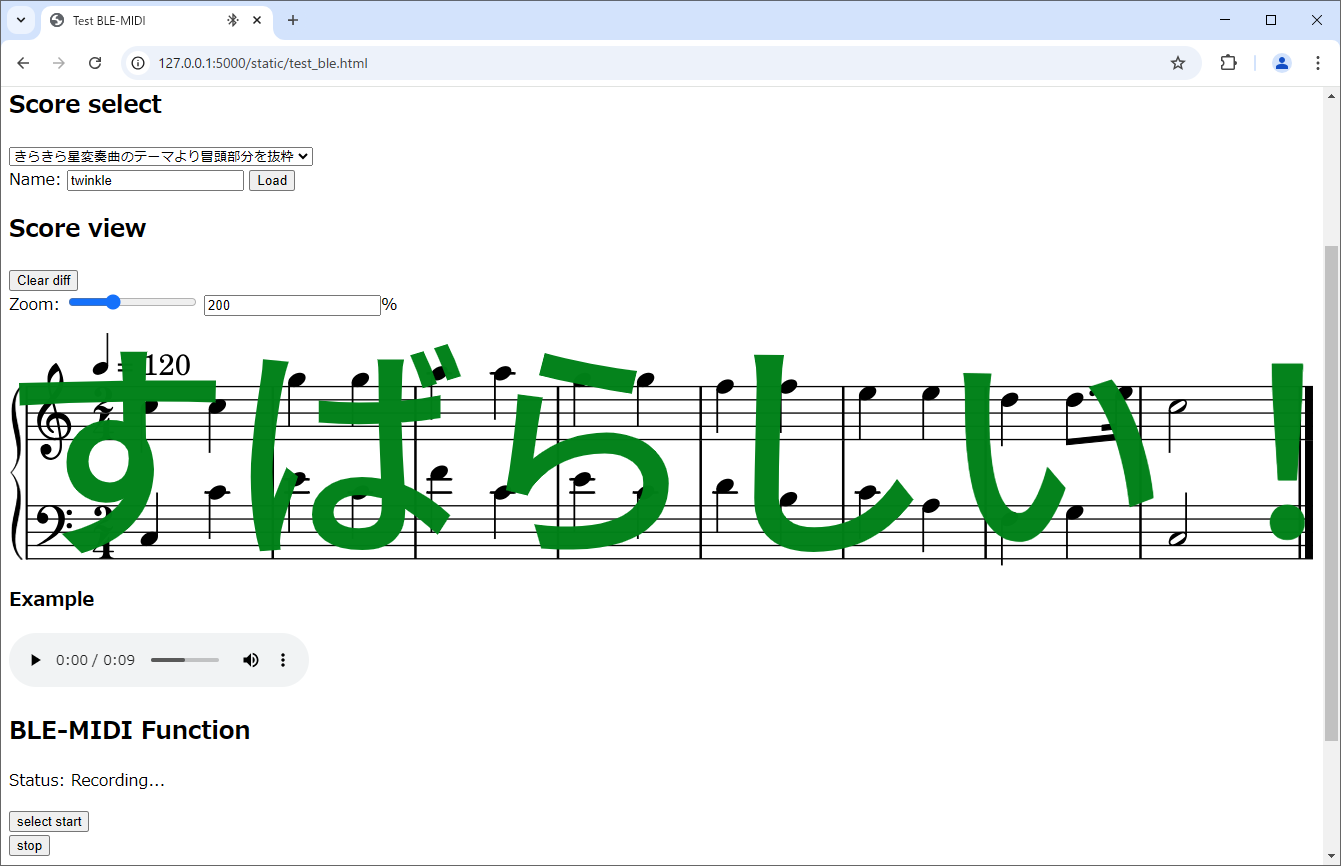
\includegraphics[width=0.7\linewidth]{twinkle-perfect.png}

  \begin{textblock*}{0.7\linewidth}(155pt,55pt)
    \onslide<*>{
      \begin{tcolorbox}[width=\linewidth,%
          left=0mm,right=0mm,top=0mm,bottom=0mm,%
          colframe=structure.fg,colbacktitle=structure.fg,%
          colback=structure.bg]
        \centering
        演奏以外の操作不要! \\
        もう一度演奏すると指摘表示が変わる
      \end{tcolorbox}
    }
  \end{textblock*}

  \begin{textblock*}{0.5\linewidth}(200pt,170pt)
    \onslide<2->{
      \begin{tcolorbox}[width=\linewidth,%
          left=0mm,right=0mm,top=0mm,bottom=0mm,%
          colframe=structure.fg,colbacktitle=structure.fg,%
          colback=structure.bg]
        \centering
        間違いがなくなれば \\
        {\bfseries\usebeamercolor[fg]{frametitle}「すばらしい!」}を表示
      \end{tcolorbox}
    }
  \end{textblock*}
\end{frame}

\section*{ポイント}

\begin{frame}\frametitle{ポイント}
  \begin{itemize}
  \item ピアノなど鍵盤楽器では楽譜(五線譜)が共通言語
    \begin{itemize}
    \item 初心者にも楽譜が読めるようになるための指導がされる
    \item 指導者や保護者にも理解しやすい
      \begin{itemize}
      \item ピアノロール表示では理解が得られない
      \end{itemize}
    \end{itemize}
  \item OSSの楽譜作成プログラムLilyPondを使用
    \begin{itemize}
    \item 表示用の楽譜画像と音符のx, y座標を同時に自動生成
      \begin{itemize}
      \item いちいち手作業で座標指定する必要が無いため省力化できる
      \end{itemize}
    \item 間違えた音符の座標に基づいて指摘を重畳表示
    \end{itemize}
  \item 楽譜と指摘表示はSVGなので拡大しても滑らか
  \end{itemize}

  \begin{textblock*}{50pt}(331pt, 110pt)
    \fontsize{10pt}{10pt}\selectfont
    \tikz{%
      \node[single arrow,fill={rgb,256:red,0;green,128;blue,0},%
        minimum height=40pt]{}
    }
  \end{textblock*}
  \begin{textblock*}{70pt}(375pt,100pt)
    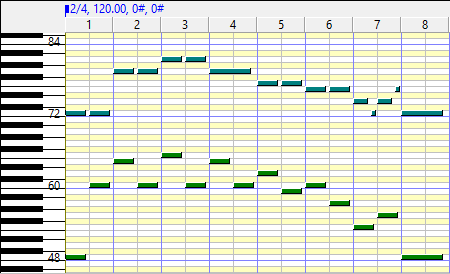
\includegraphics[width=\linewidth]{twinkle-altered-pianoroll.png}
  \end{textblock*}
\end{frame}

\section*{おわりに}

\begin{frame}\frametitle{おわりに}
  \begin{itemize}
  \item 現地参加の方はぜひShowcase会場へどうぞ
    \begin{itemize}
    \item 実際にキーボード(楽器)を演奏して試用できます
    \end{itemize}
  \item アンケートにもご協力おねがいいたします
  \end{itemize}

  \centering
  \vspace{.5\zh}
  \qrcode[hyperlink,height=100pt%
  ]{https://docs.google.com/forms/d/e/1FAIpQLSfd8qTgT6pHfkADAu4kg9s0OJLg1ycHa0GWlN5hJh9_At_UqQ/viewform?usp=header} \\
  \vspace{.5\zh}
  \fontsize{6pt}{7pt}\selectfont%
  \url{https://docs.google.com/forms/d/e/1FAIpQLSfd8qTgT6pHfkADAu4kg9s0OJLg1ycHa0GWlN5hJh9_At_UqQ/viewform?usp=header}
\end{frame}

\end{document}
